\documentclass[10pt,twocolumn]{article}
% \usepackage{silence}
% \WarningFilter{latex}{You have requested package `isqcmc2025',}
\usepackage{isqcmc2025} % Template derived from SBCM Conference

\usepackage{graphicx,url}

%\usepackage[brazil]{babel}
%\usepackage[latin1]{inputenc}

% If needed, change this to:
% \usepackage[utf8]{inputenc}

% \usepackage{lmodern}  % Load Latin Modern fonts


%%%%%%%%%%%%%%%%%%%%%%%%%%  ANONYMIZATION  %%%%%%%%%%%%%%%%%%%%%%%%%%%%%%%%%
% The anonymize.sty package facilitates double-blind peer review
% THE PAPER SHOULD BE SUBMITTED AS ANONYMOUS!!!
\usepackage[blind]{anonymize} % Blind
% \usepackage{anonymize} % Not blind
% Comment the first line and uncomment the second above to remove the black strips / blindness
%%%%%%%%%%%%%%%%%%%%%%%%%%%%%%%%%%%%%%%%%%%%%%%%%%%%%%%%%%%%%%%%%%%%%%%%%%%%
% ==== Code Listing styling ====== %
\usepackage{listings}

% Optional Custom Language definition
\lstdefinelanguage{OPENQASM}{
morekeywords={q, c}, % Primary color
morekeywords=[2]{OPENQASM, include}, % Secondary color
emph={h,cx,qreg,creg,->}, % Main emphasis color
morekeywords=[3]{measure}, % Second emphasis color
morekeywords=[4]{barrier}, % Third emphasis color
sensitive=true,
morecomment=[l]{//}, % Comment definition
morestring=[b]",
literate={->}{{\textbf{\color{codeemph2}{$\to$}}}}1 % Add emphasis for -> in this language% String definition
}


% Use this to include ORCiD Link
% \usepackage{orcidlink}
% Use \orcidlink{0000-0000-0000-0000} command after author's name and institution




\sloppy

\title{Sample Paper Using the \LaTeX\ Style for ISQCMC'25}

\author{\anonymize{First Author }\inst{1}\thanks{Supported by \anonymize{[[Sponsor]]}.} \and
        \anonymize{Second Author}\inst{1}\inst{2}}

\address{\anonymize{First Laboratory -- University/Institution}\\
         \anonymize{Street Address - Postal Code - City/Town - State/Province - Country}
         \nextinstitute
         \anonymize{Second Laboratory -- University/Institution} \\
         \anonymize{Street Address - Postal Code - City/Town - State/Province - Country}
         \email{\anonymize{first\_email@institut.de, second\_email@university.ac.uk}}
}

\begin{document}

\maketitle

\begin{abstract}
This meta-paper describes the style to be used in submissions for the 2nd International Symposium on Quantum Computing and Musical Creativity. Papers must be written in English. The abstract must be an objective text between 80 and 200 words containing a brief summary of the paper's content and research topics. It should also clearly state the contributions of the work.
Please note that \textbf{the paper should be anonymized} for submission and peer review, and in consequence, \textbf{non-anonymized papers may be atutomatically rejected}. Anonymization can be achieved by using the \lstinline[breaklines=true]!\usepackage[blind]{anonymize}! package (with the \texttt{[blind]} flag active), together with the \lstinline[breaklines=true]!\anonymize{}! command.

For example, the next sentence of this abstract should appear with a black stripe when anonymization is active: \anonymize{\textbf{This sentence contains information that should be anonymous to the peer reviewer}}

This template is derived from the SBCM 2019 conference template, which in turn was also based on a default conference template of the Brazilian Computing Society (SBC)

\end{abstract}


\section{General Information}\label{sec:gen}

All papers submitted to ISQCMC 2025 must be written in English. A typical conference paper is usually 4 to 8 pages long, although they are not strictly restricted to a maximum of 8 (as long as the content is presented in a reasonable size). 

The paper must be formatted to A4 paper, two columns, 2 cm top margin, 1.9 cm left and right
margin, 2.5 cm bottom margin and 0.81 cm separation between columns. 



\section{First Page}

The first page must display the paper title, names and addresses of the authors and the abstract. The title must be centered over the whole page, 16 points boldface font. Author names must be centered, 10 points font, boldface, all of them disposed in the same line, separated by commas. Addresses must be centered, 10 points font.
The abstract must be 10 points font, indented 0.8cm on both sides.

\section{Sections and Paragraphs}
Section titles must be in boldface, 13pt, flush left. There should be 10pt of extra space before each title. Section numbering is mandatory. All paragraphs must be indented by 1 cm.

\subsection{Subsections}

The subsection titles must be in boldface, 10pt, flush left.

\subsubsection{Subsubsection}

Subsubsections titles must be in boldface, 10pt, flush left.

\section{Figures and Captions}

Figures and tables captions should be centered if less than one line
(Figure~\ref{fig:exampleFig}), otherwise justified and indented by
0.8cm on both margins. The font must be Helvetica, 10 point, boldface, with 6 points of space before and after each caption.

In tables, do not use colored or shaded backgrounds, and avoid thick,
doubled, or unnecessary framing lines. When reporting empirical data,
do not use more decimal digits than warranted by their precision and
reproducibility.

\begin{figure}[h]
\centering
  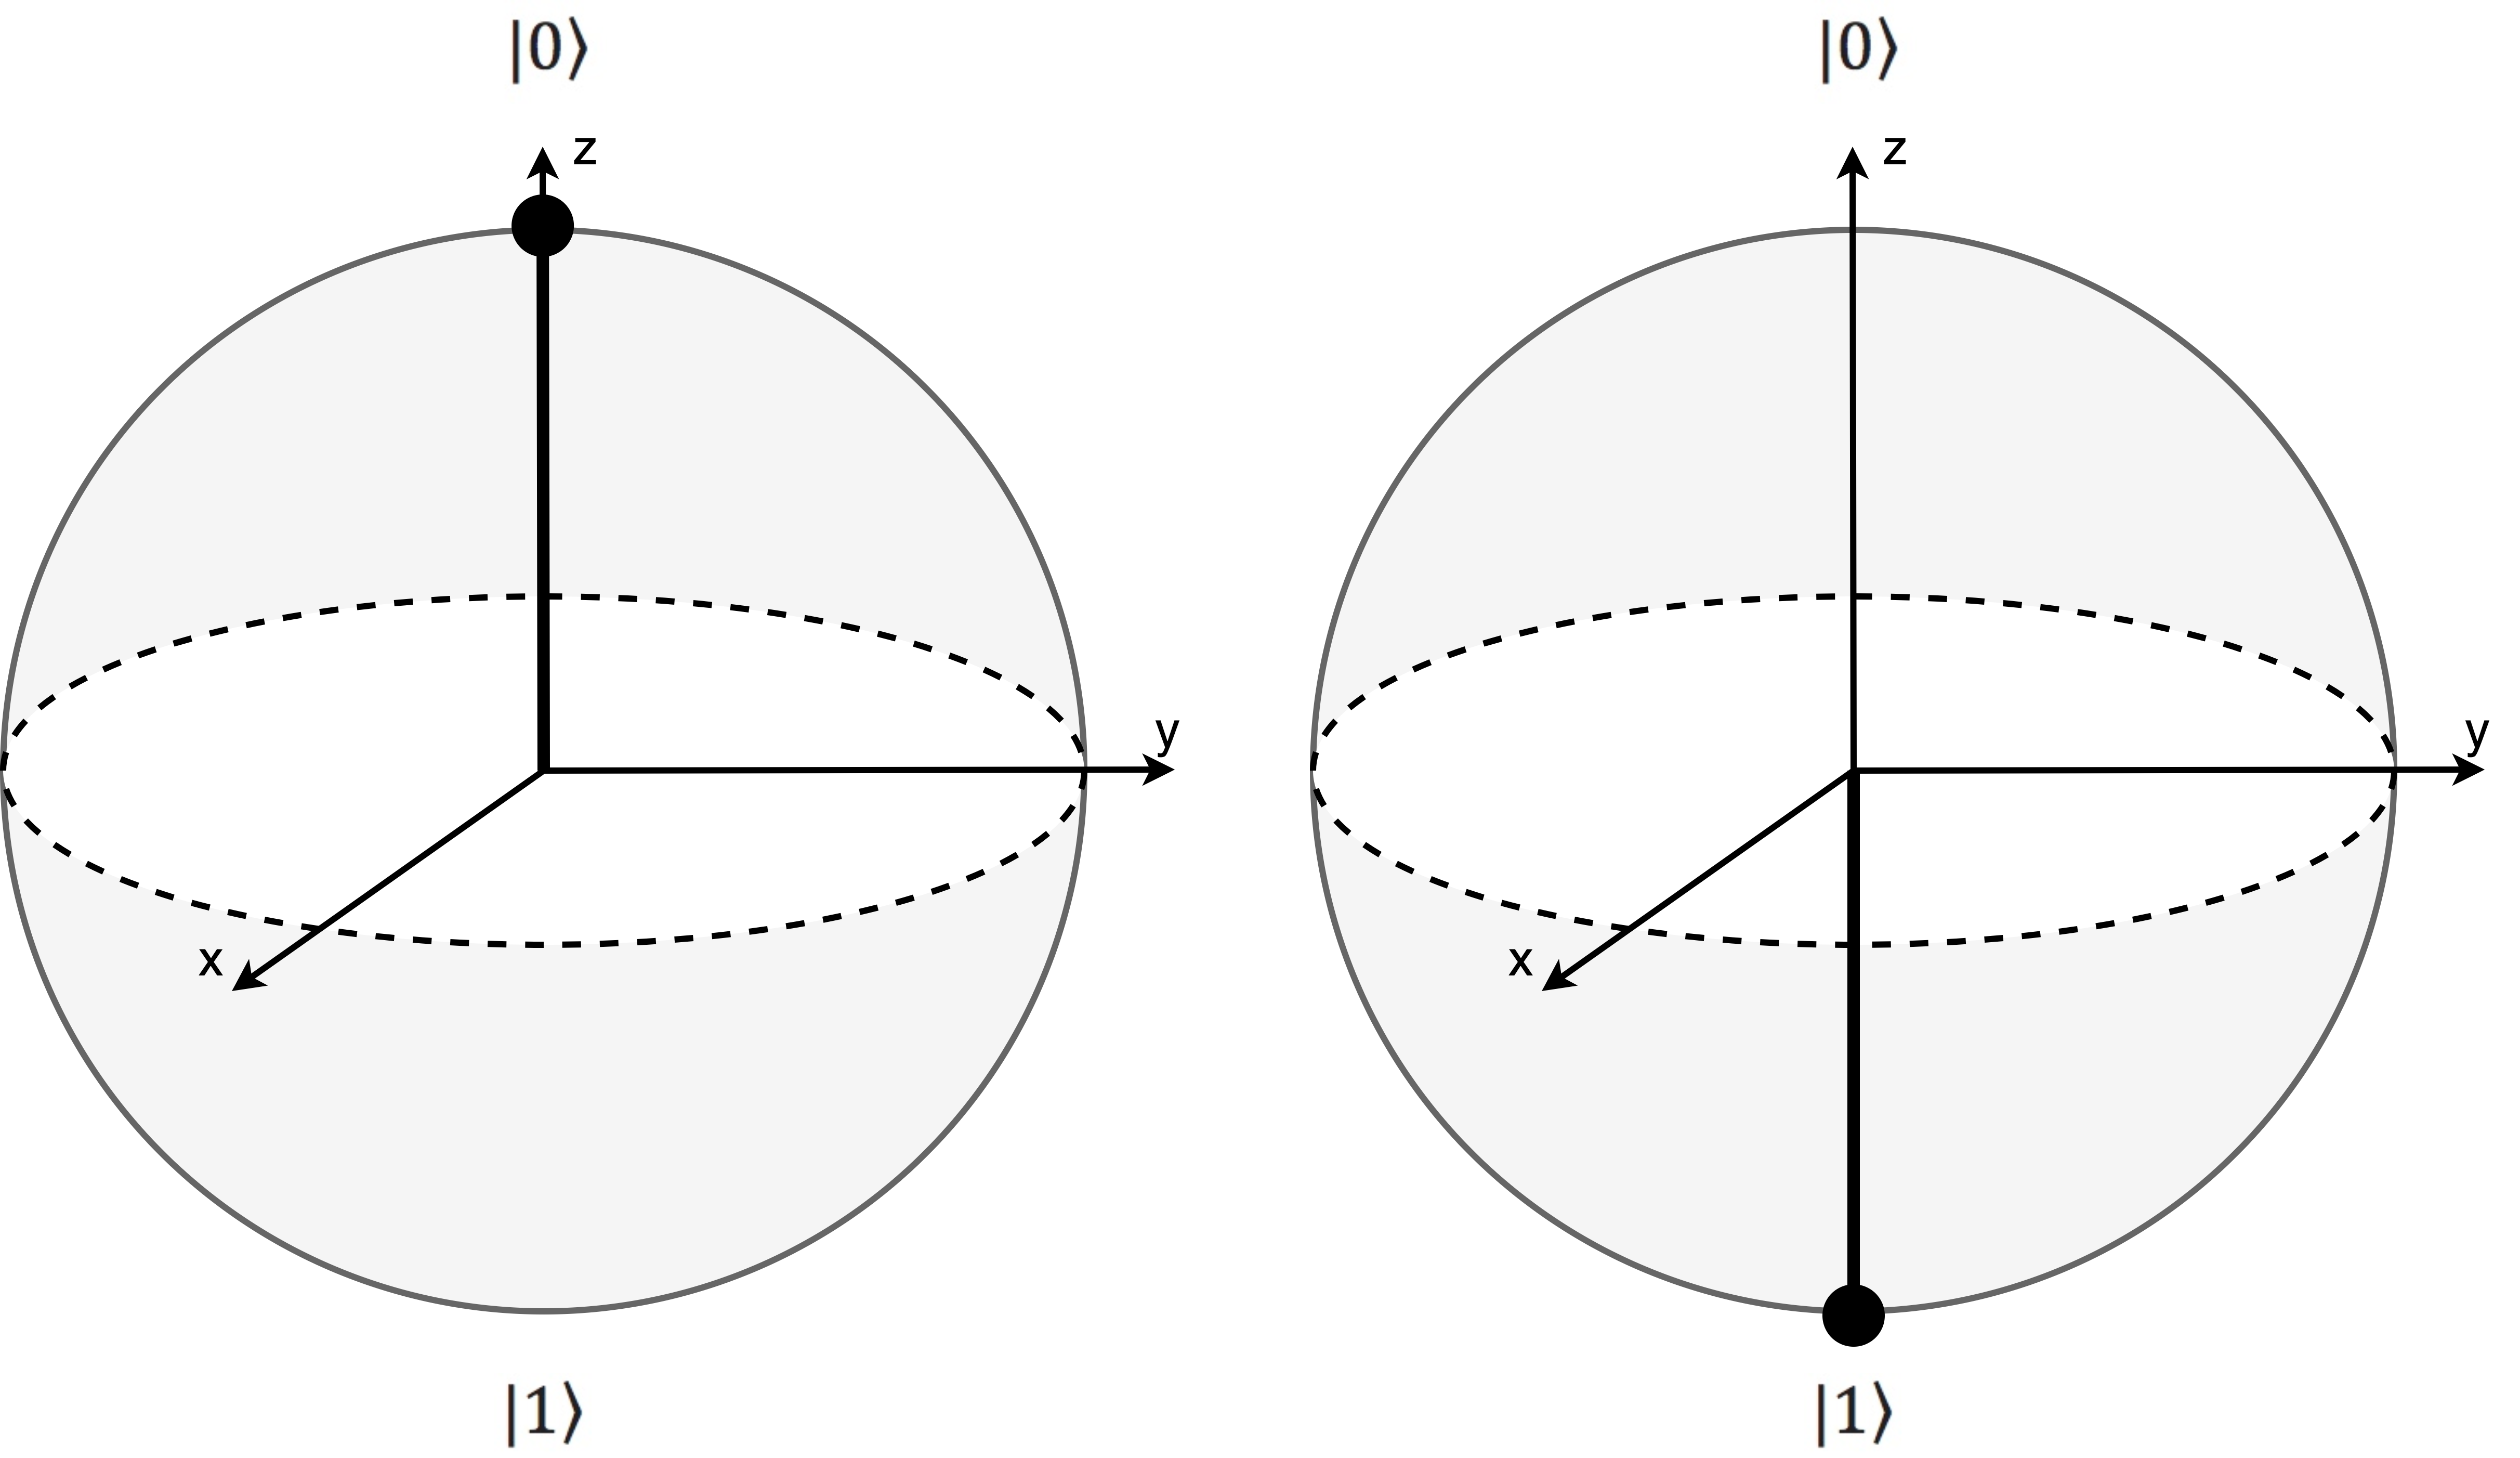
\includegraphics[width=.45\textwidth]{fig/bloch.png}
\caption{A typical figure}
\label{fig:exampleFig}
\end{figure}


\section{Images}

All images and illustrations can be in color, but they must be visible in black-and-white, or gray tones.
The image resolution on paper should be about 600 dpi for black-and-white images, and 150--200 dpi for grayscale images.

\section{Code}

Code snippets should use the \texttt{listings} package with the pre-defined ISQCMC style, as provided in the example below. Custom languages can also be defined, such as OPENQASM code depicted in Code (\ref{code1})

\footnotesize
\begin{lstlisting}[language=OPENQASM, caption=Bell Circuit,label=code1]
OPENQASM 2.0;
include "qelib1.inc";

qreg q[2];
creg c[2];

// Create Bell state
h q[0]; // Apply Hadamard gate to 1st qubit
cx q[0],q[1]; // Apply CNOT gate 

barrier q; // Special syntax highlighting defined here

// Measure the qubits
measure q -> c;
\end{lstlisting}
\normalsize

\section{References}

Bibliographic references must be unambiguous and uniform. They must be numbered in order of appearance, e.g. \cite{knuth:89}, \cite{smith:99}.


\bibliographystyle{unsrt}
\bibliography{example}

\end{document}

